\RequirePackage{fix-cm}
\documentclass[conf]{new-aiaa}

\usepackage[utf8]{inputenc}
\usepackage{hyperref}
\usepackage{graphicx}
\usepackage{siunitx}
\sisetup{group-separator = {,}}
\usepackage{booktabs}
\usepackage{enumitem}
\usepackage{float}
\usepackage{amsmath}
\usepackage[version=4]{mhchem}
\usepackage{longtable,tabularx}
\usepackage{placeins}
\usepackage{multirow}
\usepackage{booktabs}
\usepackage{latexsym}
\usepackage{subcaption}
\usepackage{latexsym}
\usepackage[sort&compress,numbers]{natbib} % For bibtex \citet, \citep
\usepackage{hypernat} % To get natbib to play nicely with hyperref
\usepackage{doi} % For getting hyperlinked DOI in the references


\hypersetup{
    pdfauthor={Peter Atma}, % insert author here
	pdftitle={Aviation 2022 Abstract}, % insert title here
	pdfsubject={Propulsion Analysis and Optimization of an Ultra Bypass Turbofan Engine}, % insert keywords here
}

\graphicspath{{../figures/}}

% [x] TODO: AL-PA, Consider changing the title to "Comparing Hydrogen and Jet-A for an N+3 Turbofan with Water Recirculation using Gradient-Based Optimization"
\title{Comparing Hydrogen and Jet-A for an N+3 Turbofan with Water Recirculation using Gradient-Based Optimization} % change
\author{Peter N. Atma\footnote{MSE Student, Department of Aerospace Engineering, AIAA Student Member}}
\author{Andrew H~.R.~Lamkin\footnote{Ph.D.~Candidate, Department of Aerospace Engineering, AIAA Student Member}}
\author{Joaquim R.~R.~A.~Martins\footnote{Professor, Department of Aerospace Engineering, AIAA Fellow}}
\affil{University of Michigan, Ann Arbor, MI, 48109}


% ==================================================
%	OVERALL COMMENTS
% ==================================================

\begin{document}

\maketitle

% ==================================================
%	Abstract
% ==================================================
\begin{abstract}
    Advances in commercial propulsion technology led to the development of efficient high bypass ratio turbofan engines with larger overall pressure ratios and internal temperatures.
    Current trends suggest that geared ultra high bypass ratio turbofans are the next generation of commercial propulsion systems.
    Furthermore, the emphasis on decreasing emissions has driven the exploration of hydrogen-powered aircraft, adding to the already challenging design space.
    % With the focus on reducing aircraft emissions, aircraft and engine manufacturers have been pushing for hydrogen as a fuel and more efficient engines to lower carbon emissions.
    Carrying and burning hydrogen introduces complexity and weight penalties that we must offset using the fuel's thermodynamic and chemical properties.
    In this study, we create a closed-loop water recirculation system with a zero-dimensional thermodynamic model and compare the benefits between jet-A and hydrogen fuels.
    We perform a gradient-based optimization parameter sweep to explore the trade-offs between performance and emissions using both fuels with water recirculation.
    The results quantify the design space for next-generation propulsion concepts that can take advantage of hydrogen fuel's advantageous thermodynamic properties to reduce emissions and improve performance.
\end{abstract}

\section{Introduction}
% Message 1: Motivation to incorporate low-emission fuels and techniques
The effects of climate change are pushing the aviation industry towards hydrogen-fueled propulsion systems as a solution to reduce emissions.
N+3 technology estimates for turbofan engines that burn hydrocarbon fuels suggest that higher efficiency can be achieved by designing ultra high bypass ratio (UHBR) engines with small cores and high overall pressure ratios (OPR).
Higher OPR and smaller cores challenge the limits of compressor and turbine design, placing an upper bound on potential performance and emissions improvements.
Switching to hydrogen as the primary fuel source reduces carbon dioxide emissions immediately, but adds complexity and weight that offset the benefits.
However, hydrogen is a versatile fuel with advantageous chemical and thermodynamic properties that can be exploited to increase the performance and reduce emissions.
We introduce a closed-loop water recirculation model that demonstrates the possible efficiency gain when hydrogen is used for purposes other than combustion.
% In this study, we investigate the tradeoff between burning hydrocarbon fuels like Jet-A versus hydrogen for UHBR ratio turbofan engines.
% We will look at new ideas with water recirculation to further squeeze performance and efficiency from Jet-A and hydrogen combustion using gradient-based design optimization.
% [ ] TODO: PA-PA, add section about MAUD and cite.

% Message 2: Background and references to support using H2 and water injection in HBTF engines
% [ ] TODO: AL-PA, Need to find a journal/conference paper to cite for the following statement.  Maybe find one or more papers other than just the NASA report?
Water recirculation is the process of extracting water from the exhaust stream of a propulsion system and injecting it upstream of the combustor as finely atomized droplets.
NASA, Boeing, and Rolls-Royce studied this concept and suggested that this technique reduces the NOx emissions as much as 47 percent~\cite{Daggett2010}.
Additionally, water recirculation improves fuel efficiency and thrust output with lower combustion temperatures that can improve the lifetime of turbine blades and reduce noise~\cite{Daggett2010}.
% [ ] TODO: AL-PA, Should try to find a citation for this if one exists.
Traditional propulsion systems that burn hydrocarbon fuels would require external water storage on the aircraft because they do not produce enough in the exhaust for recirculation.
The added weight of tanks, pumping, and ducting makes this concept infeasible for a conventional aircraft.
The main product of hydrogen combustion is water vapor and can thus be recovered from the exhaust stream.
Recirculating water vapor from the exhaust of hydrogen combustion reduces the requirement for storage tanks and allows for the creation of a closed loop system inside the propulsion cycle.

Zero-dimensional cycle modeling is an efficient tool for predicting the initial design, performance, and emissions of new propulsion concepts.
% [x] TODO: AL-AL, Need to cite CEA paper.
Zero-dimensional analysis uses a first-principles approach with a chemical equilibrium analysis (CEA) thermodynamics solver~\cite{Gordon1994} that considers the molecular species of different fuels.
% CEA can be used to understand the trends and design limitations of an engine cycle and study potential improvements in design using optimization.
The industry standard for thermodynamic cycle analysis is the Numerical Propulsion System Simulation (NPSS) framework~\cite{JonesNPSS}.
NPSS is a modular object-oriented library that models engine components as individual blocks with several thermodynamic solvers.
\citet{Hendricks2019} created a new tool called pyCycle with the same functionality as NPSS with analytical derivatives for each engine component and thermodynamic solver~\cite{Gray2017b}.
pyCycle is built on top of the OpenMDAO framework~\cite{Gray2019a} to enable gradient-based optimization and leverage hierarchical nonlinear solver structures for robustness.

% Message 3: Introduce the extension of the HBTF and propose novel contributions
In this work, we analyze the thermodynamic benefits of a closed-loop water vapor recovery and water injection system in a high-bypass turbofan engine.
We develop pyCycle components for water injection and vapor recovery to quantify the benefit of a closed loop recirculation system.
We use gradient-based optimization to minimize fuel burn subject to performance requirements using both jet-A and hydrogen at a range of flight conditions.
The optimized results show the trade-off between complexity, performance, and efficiency for jet-A and hydrogen fuels.

This work is organized as follows. First, in Section \ref{sec:method}, we introduce the turbofan model and explain the water injection and water recovery components.
In section \ref{sec:optprob} the implementation of the multipoint optimization problem is discussed.
Finally, we present the optimized results and discuss the design space in section \ref{sec:results}.

\section{Methodology}
\label{sec:method}
\subsection{Engine Model Overview}
% Engine Architecture: Describe the flow path of the engine and establish the mechanical coupling.
The UHB turbofan model is the NASA advanced technology "N+3" engine \cite{Jones2017a}.
The N+3 reference cycle represents a UHB ratio geared turbofan that could be available in the 2030 to 2040 time frame.
% We selected the N+3 model because it has already been modeled in pyCycle as a robust example cycle and includes the advanced engine cycle improvements such as a large bypass ratio, high pressure ratio, and high combustion temperature.
The flow path consists of an inlet that directs ambient air through a fan, followed by a duct that splits the flow into a core and a bypass stream, each ending in a core and bypass nozzle, respectively.
The low pressure system is split into two mechanical subsystems.
First, the fan is connected to the gearbox that reduces the shaft speed to decrease the fan tip speeds.
Second, the gearbox attaches to the low-pressure shaft that connects to the low-pressure compressor (LPC) and low-pressure turbine (LPT).
% The low pressure system consists of a fan connected to a gearbox that attaches to the lo and low pressure compressor (LPC) are connected to the low pressure turbine (LPT) by the low pressure shaft.
The high pressure compressor (HPC) is connected to the high pressure turbine (HPT) by the high pressure shaft.

% [ ] TODO: AL-PA, potentially move the commented line below about CEA into the subsection discussing the propulsion model.  I think it's too much detail for the setup of this section.
% Thermodynamic equations of state are solved using CEA at the interface between components, shown as black arrows in Figure~\ref{fig:n3_cycle}.
We introduce the closed-loop water recovery system as a feedback loop that transports water from the exhaust to upstream of the compressors.
% The closed-loop water recovery system is implemented into the cycle by placing a water injection component directly before the HPC.
The recovery system injects vaporized water into the core stream that reduces the combustion temperature due to heat absorption.
The vapor recovery component is placed directly before the core nozzle to extract water from the exhaust and recycle it back to the injector.
% NOTE: AL-PA, don't discredit your work before you even explain the model and methods.  We can make this point in the results or conclusion.
% In practice a water vapor recovery component requires a complex condenser model in the core stream, this work will only look at the potential benefits of extracting water vapor and not the recovery method specifically.

In this section we explain the implementation and assumptions of the water recovery model.
We present the full engine layout and provide details on the multipoint zero-dimensional modeling approach.
The component flow interface and mechanical connections, including the water injector and water extractor, are depicted in Figure \ref{fig:N3_original}.
% The propulsion model is constructed in pyCycle which is built on top of OpenMDAO to allow a modular design of the engine components and the coupling of other engineering disciplines for analysis \cite{Gray2019a}.
% The engine model that was selected for this project is the NASA advanced technology UHB geared turbofan engine cycle, referred to as the "N+3" engine \cite{Jones2017a}.
% The N+3 reference cycle represents a UHB ratio geared turbofan that could be available in the 2030–2040 time frame and was selected since it has already been modeled in pyCycle as a robust example cycle and includes the advanced engine cycle improvements such as a large bypass ratio, high pressure ratio, and high combustion temperature.
% The flow path consists of an inlet that directs ambient air through a fan, followed by a duct that splits the flow into a core flow and a bypass flow, each of which ends in a bypass nozzle and core nozzle, respectively.
% The fan and low pressure compressor (LPC) are connected to the low pressure turbine (LPT) by the low pressure shaft and the high pressure compressor (HPC) is connected to the high pressure turbine (HPT) by the high pressure shaft.
% Along the axial flow path, the zero-dimensional thermodynamic connections are solved using CEA to ensure the first principle governing equations are satisfied.
% Figure \ref{fig:N3_original} shows how the 25 elements in the N+3 cycle are connected together with the fluid flows in blue, the mechanical connections in red, and the performance elements in green \cite{Hendricks2019}.

% [ ] TODO: AL-PA, Remove the black box with the component descriptions from the bottom left of the figure.
% [ ] TODO: AL-PA, Add the description of the figure elements to the caption.
% [x] TODO: AL-PA, Consider changing the caption to "Simplified layout of the N+3 engine cycle, adapted from~\citet{Hendricks2019}"
% [x] TODO: AL-PA, Remove the flight conditions component and add the bypass duct component below the splitter. I think the bypass is an important enough aspect of the engine to include.
\begin{figure}[hbt!]
    \centering
    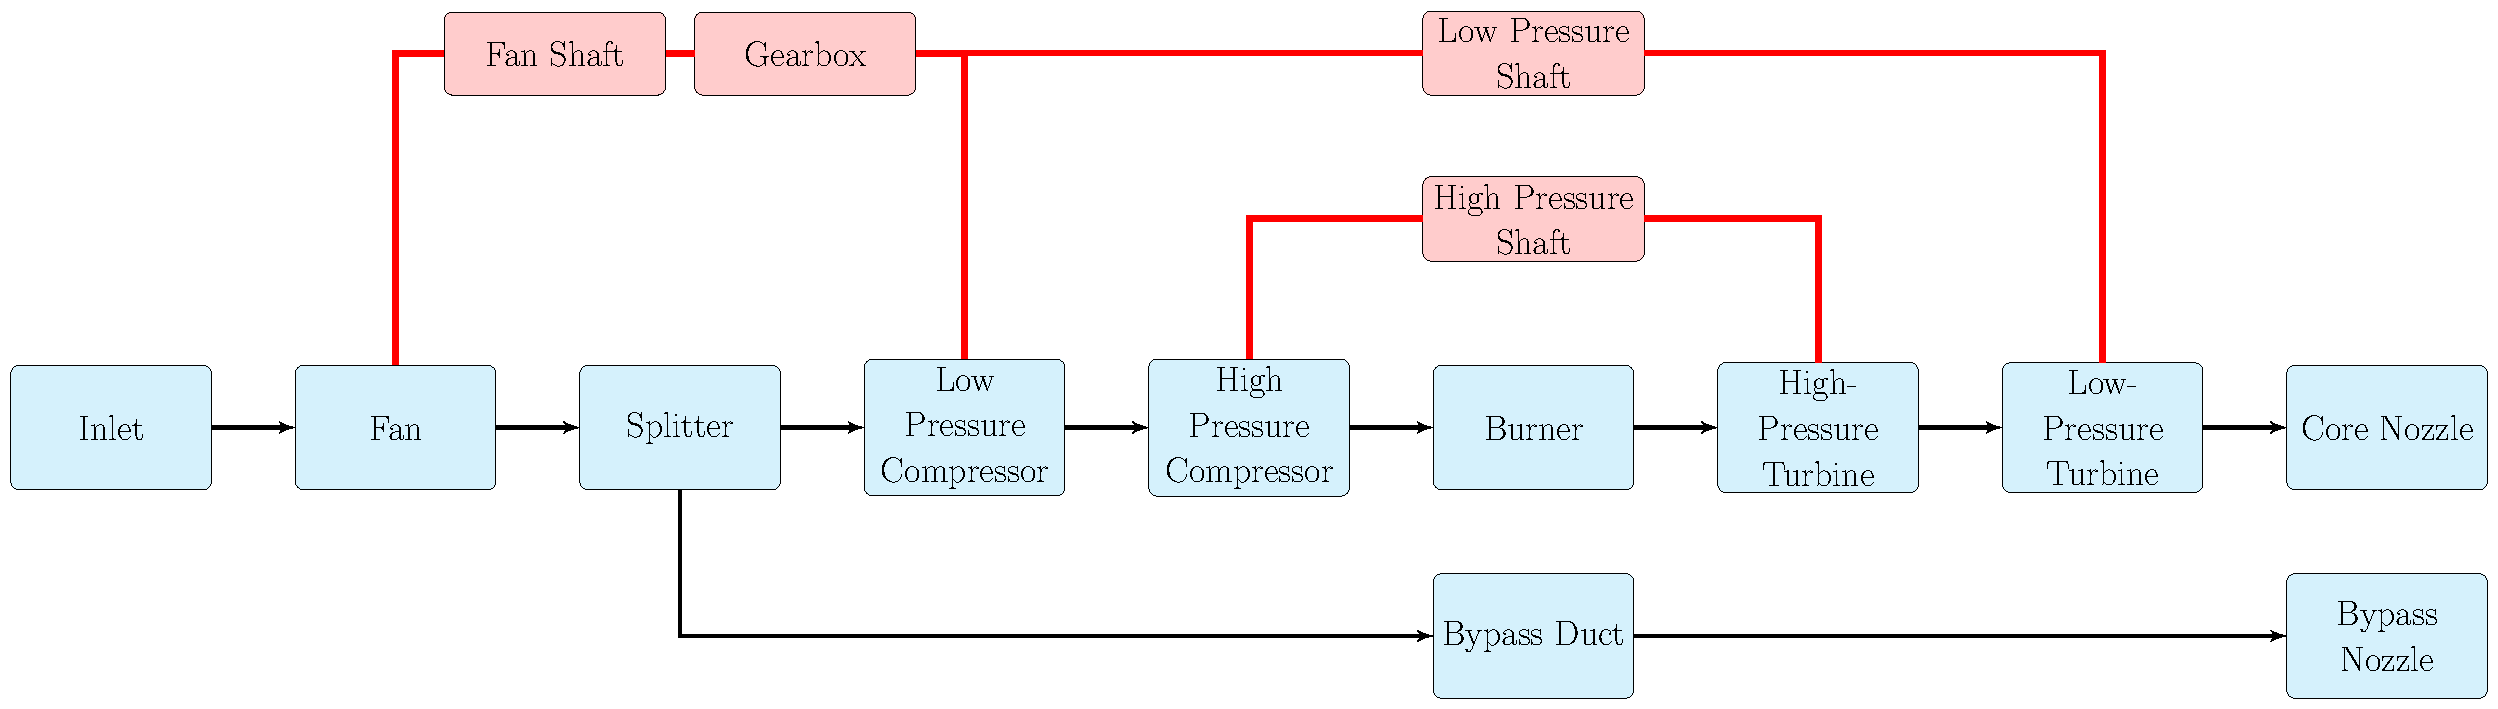
\includegraphics[width=1.0\textwidth]{N3_cycle.pdf}
    \caption{
        Simplified layout of the N+3 engine cycle, adapted from~\citet{Hendricks2019}.
        Black arrows are flow connections, red lines are mechanical connections, blue boxes are cycle elements, red boxes are shaft elements.
    }
    \label{fig:N3_original}
\end{figure}

\subsection{Water Recovery Model}
We implemented the closed-loop water recovery system as a feedback system that extracts water from the exhaust stream and injects it upstream of the HPC.
% The closed-loop water recovery system is implemented into the cycle by placing a water injection component directly before the HPC.
% This component will inject pure water into the core stream which will reduce the combustion temperature due to heat absorption from vaporization.
We chose this injection location based on claims from a study by NASA, Boeing, and Rolls-Royce~\cite{Daggett2010} that water injection directly into the combustor is unnecessary.
% This location was chosen as it was one of the configurations chosen by the aforementioned NASA, Boeing, and Rolls-Royce study that did not require direct combustor injection \cite{Daggett2010}.
The water vapor recovery component sits downstream of the LPT and extracts water from the flow before it exits the core nozzle.
% The water vapor recovery component is placed directly before the core nozzle to extract water from the core stream and recycle it back to the water injector.
% Water is recovered from this location as it is the last possible location before the nozzle in which water can be extracted.
% [ ] TODO: AL-PA, add a sentence about the assumptions for the vapor recovery instead of the mentioning the condenser
% NOTE: AL-PA, we will talk about the condenser when we discuss the results of the pressure recovery parameter sweep.
% In practice a water vapor recovery component requires a complex condenser model in the core stream, this work will only look at the potential benefits of extracting water vapor and not the recovery method specifically.
The component flow interface and mechanical connections, including the water injector and water extractor, are depicted in Figure \ref{fig:n3_cycle}.

\begin{figure}[hbt!]
    \centering
    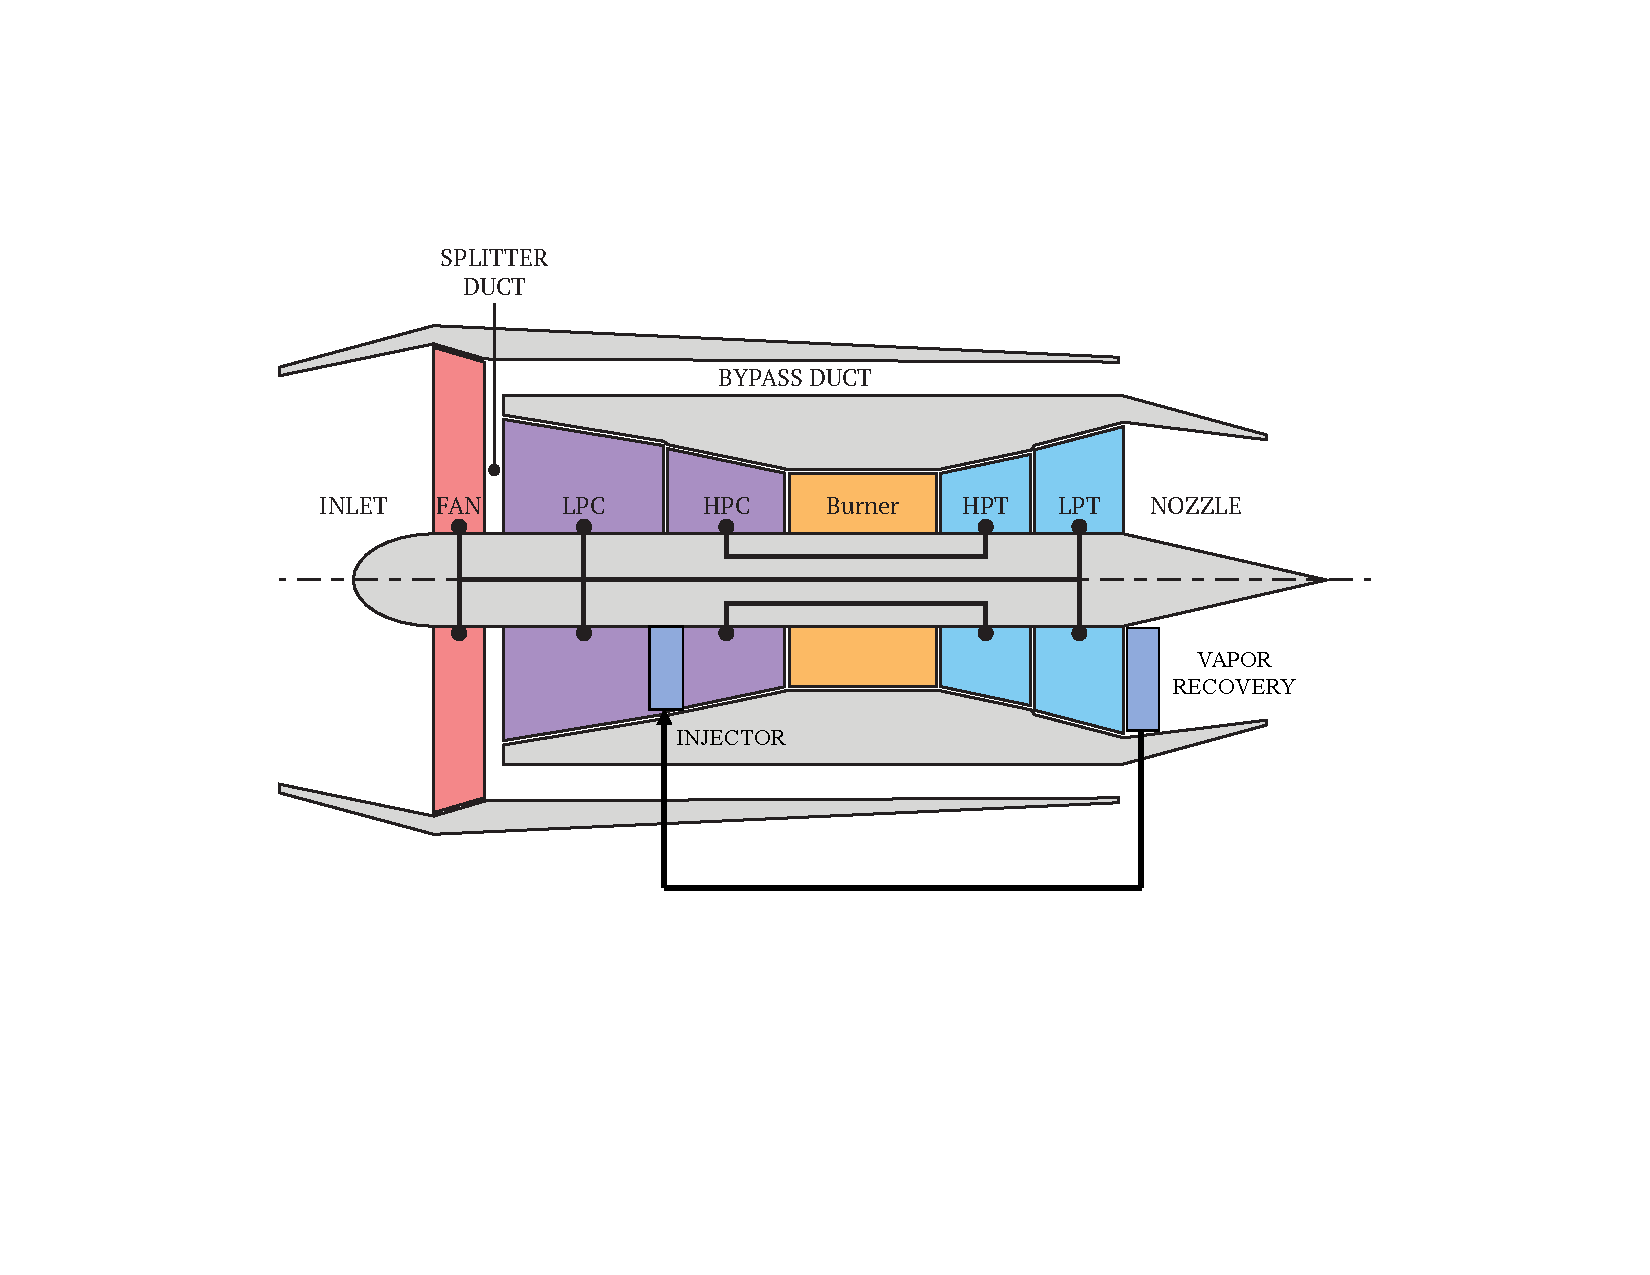
\includegraphics[width=0.75\textwidth]{turbofan_wvr.pdf}
    \caption{
        The configuration of a high-bypass turbofan model with an integrated closed-loop water vapor recovery and injection system.
        The water vapor recovery system (extractor) extracts a fraction of the water in the core stream and reinjects it upstream of the high-pressure compressor.
        This diagram illustrates the feedback effect that this implementation has on the overall core flow.}
    \label{fig:n3_cycle}
\end{figure}

We modified the composition of the air mixture upstream of the combustor to account for humidity.
% Since water is being used in the sections of the engine upstream of the combustor, this model was designed to take the humidity of the air into account.
% To utilize water engine section infront of the combustor the N+3 engine model had to be modified to include $H_2O$ as a species.
pyCycle provides a \texttt{wet-air} dataset that introduces $\mathrm{H_2O}$ molecules to the composition of air.
% The \texttt{wet-air} dataset inherits the NPSS \texttt{JANAF} data from the original model but removes a couple troublesome hydrocarbons from the product species as they can cause numerical issues.
% The FlightConditions() pyCycle subsystem can then have a reactant and mixture ratio specified when implemented.
We prescribe atmospheric mass-specific humidity as a water-to-air ratio (WAR) that is defined as the ratio of $\mathrm{H_2O}$ to air in the reactants of the inflow mixture.
% In this case, the reactant is be $H_2O$ and the mixture ratio is the water-to-air (WAR) ratio of the water content in the air.
% The WAR is the sp of the air expressed in equal units and separating out the total mass (kg water/kg air).
\citet{Kalnay1996} give the humidity values for each flight condition.
% The humidity values used in this paper are from a NOAA dataset \cite{Kalnay1996}.

We introduce two new thermodynamic models for water recirculation in pyCycle.
% To model the complicated water recirculation loop in pyCycle new components had to be developed.
A water injector adds water to the flow upstream of the HPC, while a water extractor diverts a portion of the water in the flow away from the exhaust stream.
% The two models are a water injector that adds water to the flow upstream of the HPC and a water extractor to divert a fraction of the water in the flow away from the exhaust stream.
The injector operates similarly to fuel injection in the combustor.
We determine a WAR that is analogous to the fuel-to-air (FAR) ratio in the combustor.
% The injector component is based on the combustor component already included in pyCycle which operates by injecting a given fuel-to-air ratio (FAR) or fuel flow rate to determine the mass of fuel added to the incoming flow.
This WAR is used to compute the chemical species present in the flow at the current thermodynamic state, determined by the incoming flow.
The new species composition and thermodynamic state are determined using the pyCycle CEA solver~\cite{Gray2017b}.
% Once the new composition is determined, the various thermodynamic variables are passed to the next component in the engine.
% The water injector component would inject water as a reactant instead of the fuel as the combustor would.
The water injector inputs are the mass flow rate and mass fraction of water.
We can solve for the mass flow rate on a mixture basis using the WAR, or directly by specifying the mass flow rate of water.
% The water injector can take either water-to-air ratio (WAR) or water mass flow rate to determine how much water is added to the flow.
A schematic of the injector is shown in Figure \ref{fig:injector} where $Y_{H_2O}$ is the mole fraction of water molecules.

\begin{figure}[hbt!]
    \centering
    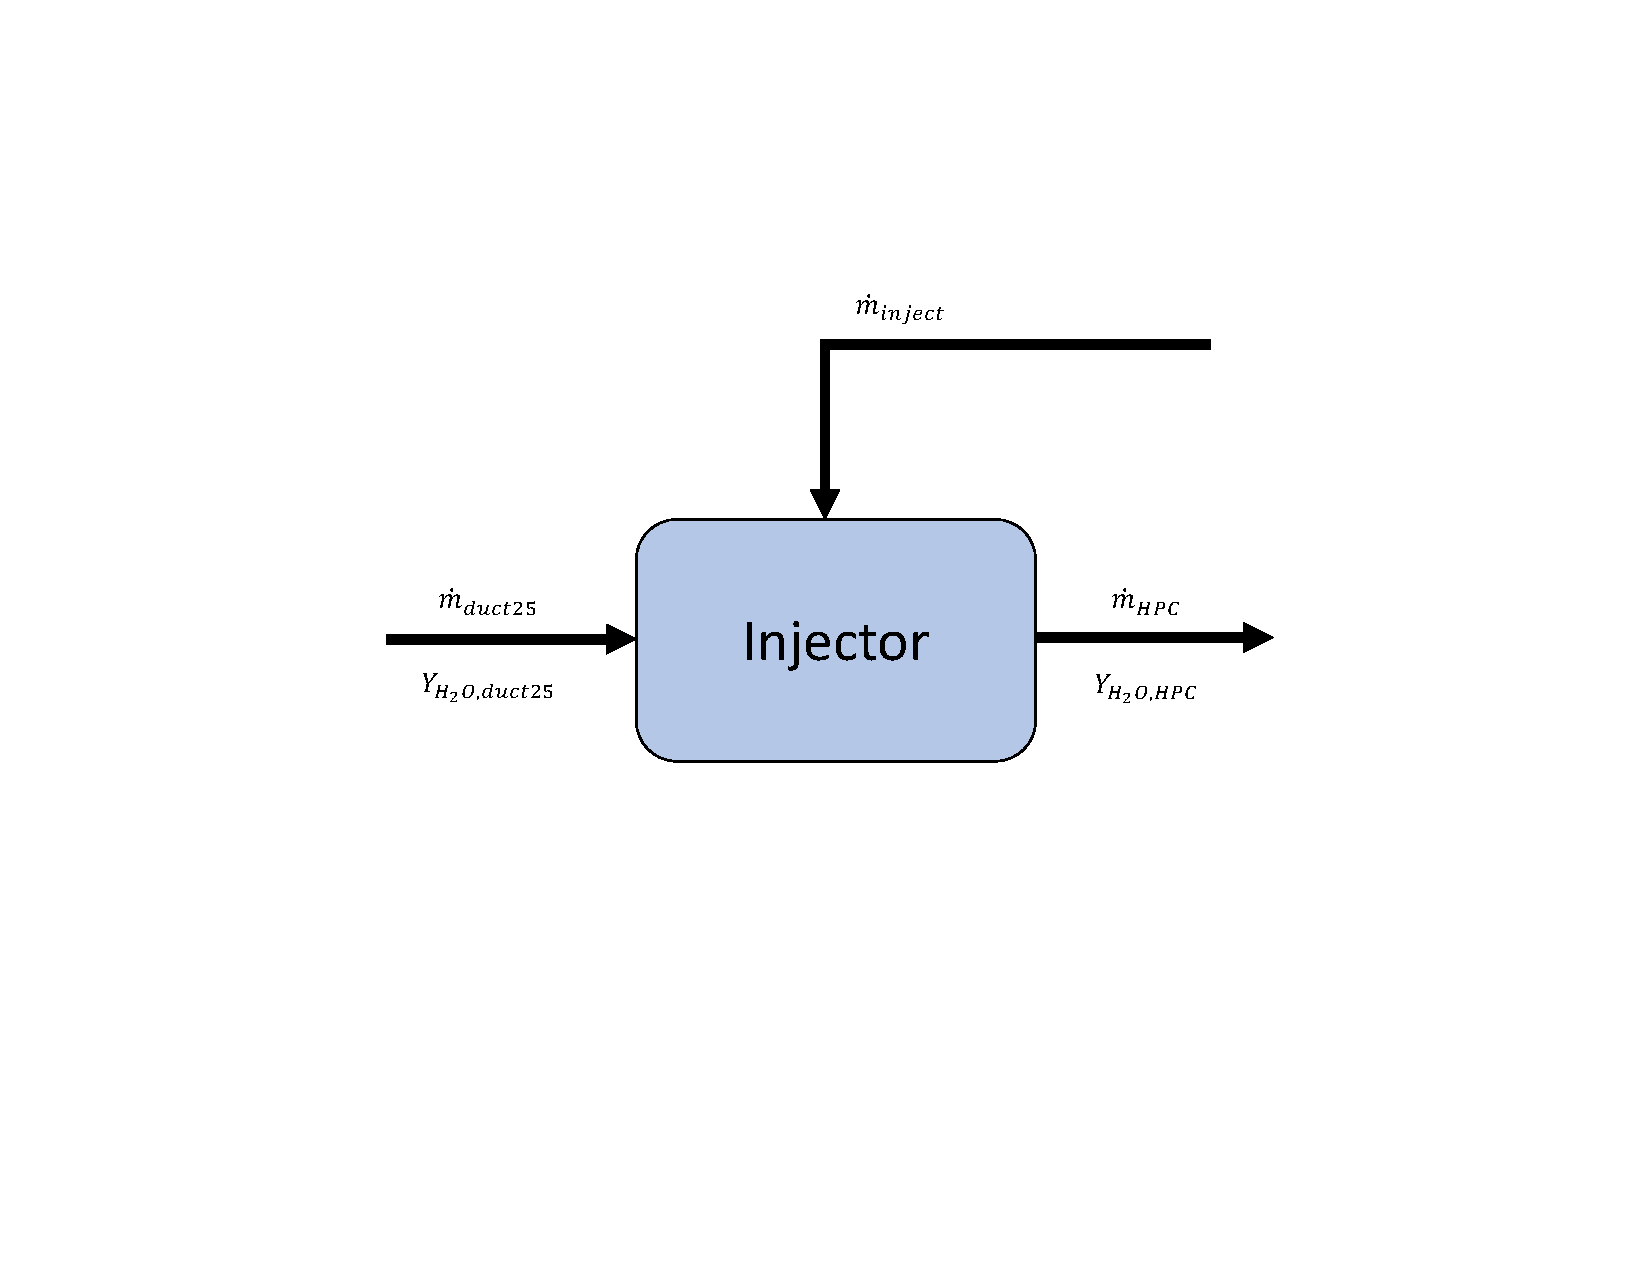
\includegraphics[width=0.75\textwidth]{injector.pdf}
    \caption{
        Injector component schematic.
        Water from the extractor is simply injected into the core flow upstream of the high-pressure compressor.
    }
    \label{fig:injector}
\end{figure}

The water extractor model diverts a fraction of a specific species from one flow path to another.
% The water extractor model is based on an air-bleed component in pyCycle with the added complexity of extracting a fraction of a specific species within the flow.
The CEA solver calculates the inflow composition and the extractor separates a specific species based on a mass fraction input.
The composition of the core stream is updated to represent the remaining mixture after the extractor model removes the desired species from the incoming flow.
We then solve for the thermodynamic state and flow path areas at the outflow of both extractor streams.
% The extraction determines the water content of the incoming flow and extracting a given fraction of that water flow.
% The water content of the incoming flow is determined by solving a CEA analysis of the incoming flow.
% This water content in the incoming flow is then used with a given fraction of the water to extract to determine the how much water mass flow to remove from the stream.
% The outputs of the extractor component are the flow rate of the core flow and the corresponding flow properties in addition to the extracted water mass flow rate.
% While this process certainly would have pressure loss penalties in terms of condensing water in a condenser, this project just looks at the effects of water recovery since there are no current models for nozzle exhaust condensers available.
A simple schematic of the extractor is shown in Figure \ref{fig:extractor} where $Y_{H_2O}$ is the mole fraction of water molecules and $X_{H_2O,k}$ is the fraction of water that is recovered from the core stream.

\begin{figure}[hbt!]
    \centering
    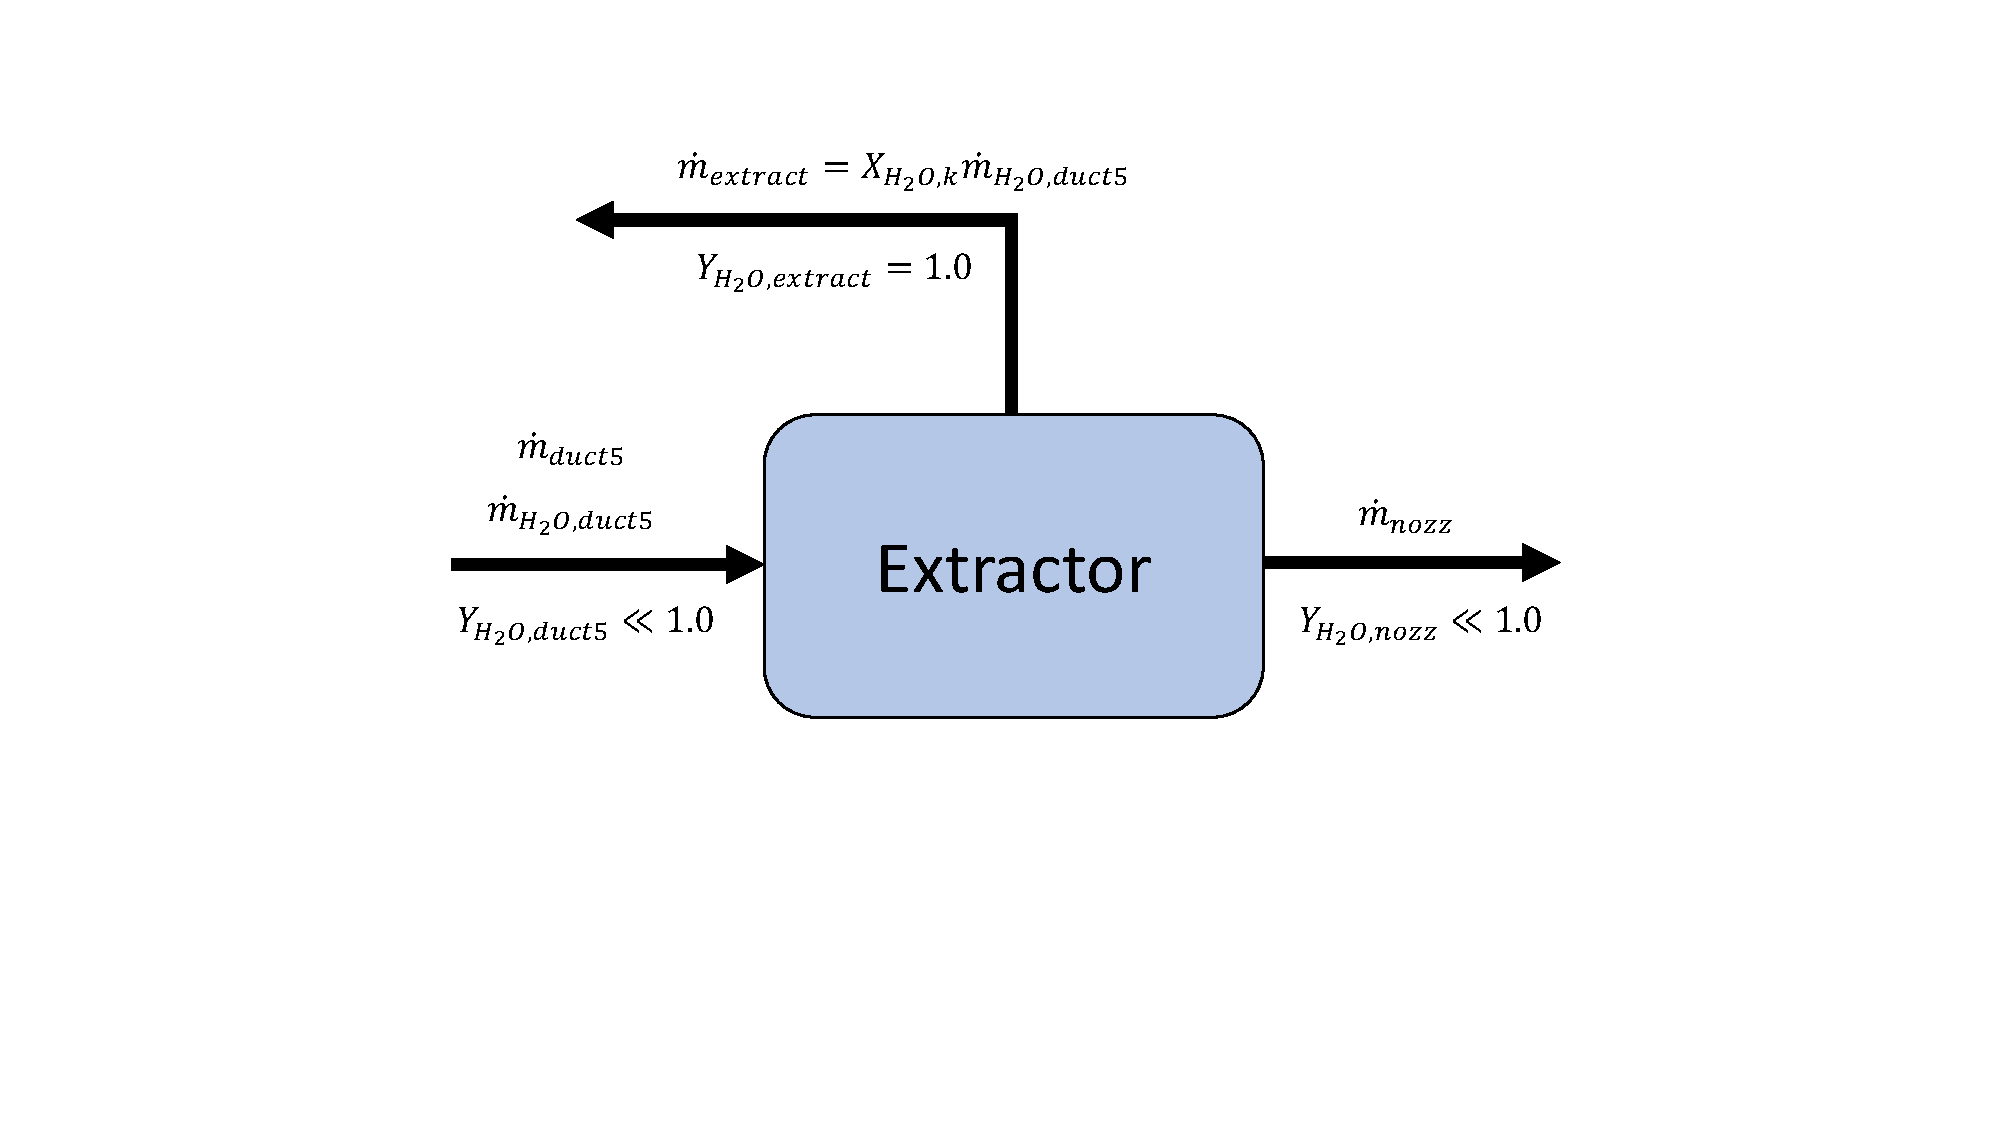
\includegraphics[width=0.75\textwidth]{extractor.pdf}
    \caption{
        Extractor component schematic.
        A certain mole fraction of the flow coming out of duct5 is comprised of water of which a certain specified fraction is extracted.
        The extracted water is routed back upstream to the injector and the rest is simply exhausted out the nozzle.
    }
    \label{fig:extractor}
\end{figure}

We connect one outflow stream of the extractor to the inflow stream of the injector to complete the water recirculation system.
The model results in a mismatch between the mass flow rate upstream of the HPC and the mass flow rate exiting the core nozzle.
To preserve conservation of mass, we treat the water recirculation as a nonlinear cycle that must converge before the engine calculation is physically balanced.
% This is because the pyCycle model is solved sequentially component to component during each Newton iteration.
% So a Nonlinear Block Gauss-Seidel solver would be sufficient to solve this feedback loop.
% However, the N+3 model already has a nonlinear Newton solver at the Multipoint Design level, so the extractor mass flow rate and injector mass flow rate variables are connected for each design point and use this nonlinear solver to converge the water streams.
We illustrate the water recirculation loop and the nonlinear solver connections in Figure \ref{fig:N3_xdsm_full}.

\begin{figure}[hbt!]
    \centering
    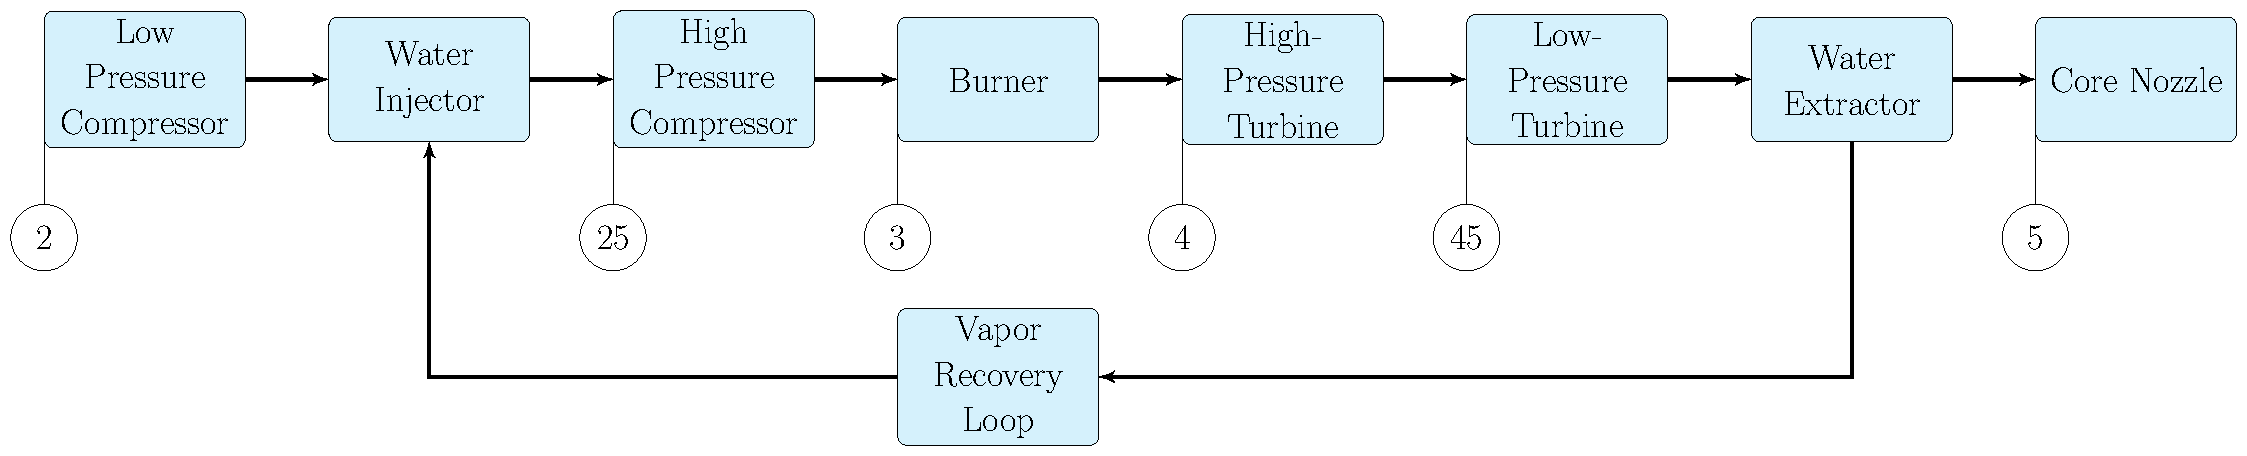
\includegraphics[width=1.0\textwidth]{N3_CLVR_cycle.pdf}
    \caption{
        Simplified layout of the N+3 engine cycle with the closed-loop vapor recovery.
        Black arrows are flow connections, red lines are mechanical connections, blue boxes are cycle elements, red boxes are shaft elements.
    }
    \label{fig:n3_clvr}
\end{figure}

In pyCycle, the Cycle block contains all of the governing thermodynamic equations needed to model an engine such as CEA analysis, compressor and turbine models, and equations of state.
These equations allow any arbitrary engine design to be assembled using the modular cycle elements.
The Cycle block itself may not result in a valid model of the engine since some physical dependencies may not match.
These physical dependencies are handled by the Balance block which solves a set of implicit state variables and nonlinear physical residual equations in the form:

\begin{equation}
    \mathcal{R}_c = \sum_{i=1}^{n} x_i = 0
\end{equation}

\noindent
where $x_i$ is some physical variable such as a mass or energy flow rate.
These residuals represent the physical conservation laws such as mass flow rate are converged to zero by the Solver.
In pyCycle, a direct solver is used for linear equations and a Newton solver is used for nonlinear equations which utilizes the analytic partial derivatives provided by each OpenMDAO component.
All residuals within the engine model are converged at the Cycle level for a given operation condition since all of the parameters downstream do not directly effect those upstream.
However, with introducing the extractor and injector components, we add a feedback loop into the model where mass is removed downstream and added upstream.
Therefore, the mass flow rates residuals of the closed-loop vapor recovery system shown below would need to be converged in the Multipoint Cycle explained in the next section.

\begin{equation}
    \mathcal{R}_{c,\dot{m}} = \dot{m}_{extractor} - \dot{m}_{injector} = 0
\end{equation}

\subsection{Multipoint Model}
The N+3 engine model as it is implemented in pyCycle has many complex thermodynamic and performance connections between different operating conditions.
Therefore, the N+3 engine model computes the engine performance at 4 different operating conditions in order to resolve the complexities between each operating condition on the final design.
The operating conditions that considered are top-of-climb (TOC), rotating takeoff (RTO), sea-level static (SLS), and cruise (CRZ).
The SLS condition represents the static performance requirements for the engine, the RTO condition represents the performance and cooling requirements at the point of rotation during takeoff, the TOC operating condition represents the performance requirements during a climb, and the CRZ operation condition represents the criuse performance of the engine.
To account for each of these operating conditions, the N+3 model uses a technique called Multipoint Design Point (MDP) modeling to converge the model to an engine design that satisfies the requirements at each of these operating conditions.
One of these operating conditions is specified as the design point, which in this case is TOC, and the other operating conditions are considered the off-design points.
The design point for the model generally sets all of the engine sizing such as areas and pressure ratios across components.
The off-design points are essentially the size of the engine at the design point but operating at the corresponding required thrust, cooling, and environmental conditions.
The design point of the engine model is converged using a linear Newton solver which then passes the geometric sizing variables such as cross-sectional areas and map scalars to the off-design points and similarly converges those.
Then, a nonlinear Newton solver is used to converge the overall model with respect to the variable connections between each operating condition.
An XDSM diagram of the nominal N+3 engine model is shown in Figure \ref{fig:N3_xdsm} \cite{Hendricks2019}.

\begin{figure}[hbt!]
    \centering
    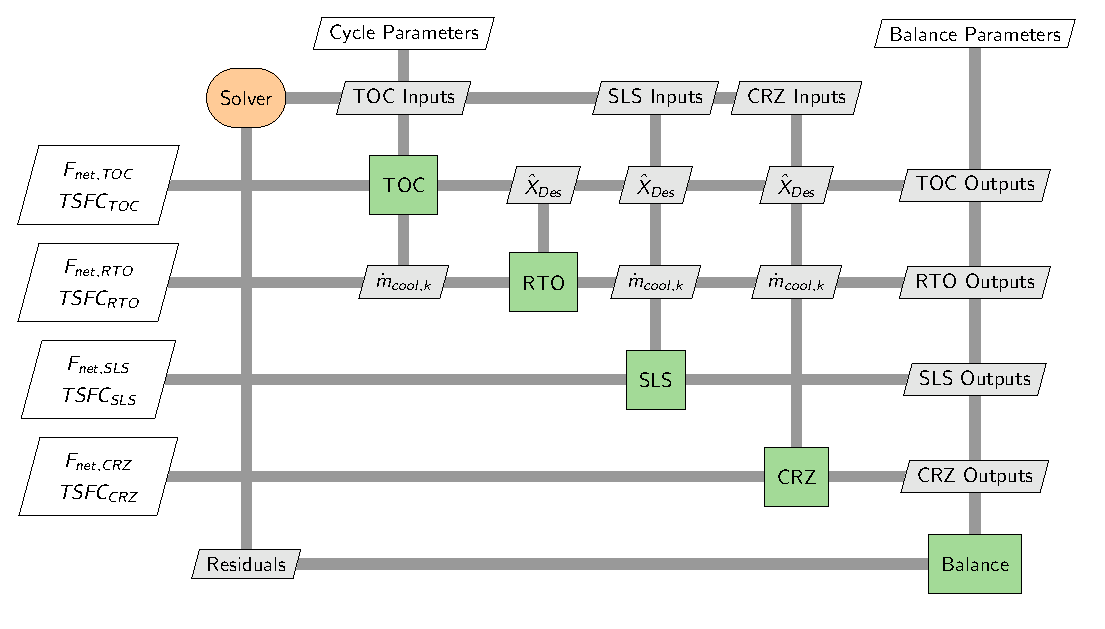
\includegraphics[width=0.75\textwidth]{N3_xdsm.pdf}
    \caption{
        N+3 engine multipoint setup XDSM diagram.
        This XDSM diagram shows how each of the operating conditions is coupled with each other and how the outputs are computed.
    }
    \label{fig:N3_xdsm}
\end{figure}

In the optimization problem described later, we set the mass flow rate of fuel, $\dot{m}_{fuel}$, as the objective function.
Our comparison metric is $TSEC_{CRZ}$ but minimizing $\dot{m}_{fuel}$ is a better posed optimization problem since we will also have thrust constraints.
Therefore, the water mass fraction that will most impact the objective function the most is at the CRZ operating condition and we thus want to size the area of the injector and extractor at CRZ instead of TOC like the rest of the areas are.
Normally, the cross-sectional areas are set at the design point (TOC) and are connected to the off-design points.
To size the areas of the injector and extractor at CRZ, we only connect the state variables across these components at the corresponding operating condition and set the areas of both components at the CRZ point.
These connections are shown graphically in the XDSM diagram in Figure \ref{fig:N3_xdsm_full}.

% Explain Exit ratios and how BPR and OD net thrusts are set
In the N+3 model implementation presented in the pyCycle paper, the bypass ratio (BPR) at TOC is computed using a Balance component.
The Balance component for $BPR_{TOC}$ uses the exit velocity ratio of the core and bypass nozzles which is given as:

\begin{equation}
    V_{ratio} = \frac{V_{core,ideal}C_{v,core}}{V_{bypass,ideal}C_{v,bypass}}
\end{equation}

\noindent
where $V_{ideal}$ is the exit velocity of a nozzle and $C_v$ is the velocity coefficient of the nozzle which represents non-ideal effects.
This adds a constraint where the core exit velocity is higher than the bypass exit velocity.

\subsection{Performance Metrics}
Past implementations of engine cycles and example engine cycles in pyCycle generally have used either JetA or JP-7 as a fuel.
However, in this work we are interested in comparing the performance of similar engines with different types of fuel, specifically hydrogen due to the many benefits it offers in terms of performance and thermal properties.
Fortunately, pyCycle comes ready to use hydrogen with cataloged exhaust products for hydrogen fuel.
The fuel type is simply changed from Jet-A to H2 in the pyCycle model.

For measuring the efficiency of jet engines, thrust-specific fuel consumption (TSFC) is generally used since it is a represents how low the fuel burn is for a given level of thrust.
However, when comparing Jet-A and hydrogen fuels this is not such a good metric since a given mass flow rate of hydrogen has an energy content almost 3 times that of Jet-A.
% TODO: Update mdolab.bib
Therefore, a new metric for comparing the relative efficiencies of engine running on Jet-A versus hydrogen is thrust-specific energy consumption (TSEC) which multiplies TSFC by the lower heating value (LHV) of the fuel %\cite{Adler2023}.

\begin{equation}
    TSFC = \frac{\Dot{m}_{fuel}}{F_{thrust}}
\end{equation}

\begin{equation}
    TSEC = \frac{\Dot{m}_{fuel} LHV}{F_{thrust}} = TSFC \times LHV
\end{equation}

With all of the sub-models of the N3 engine presented, the complete engine cycle XDSM diagram is shown in Figure \ref{fig:N3_xdsm_full}.

\begin{figure}[hbt!]
    \centering
    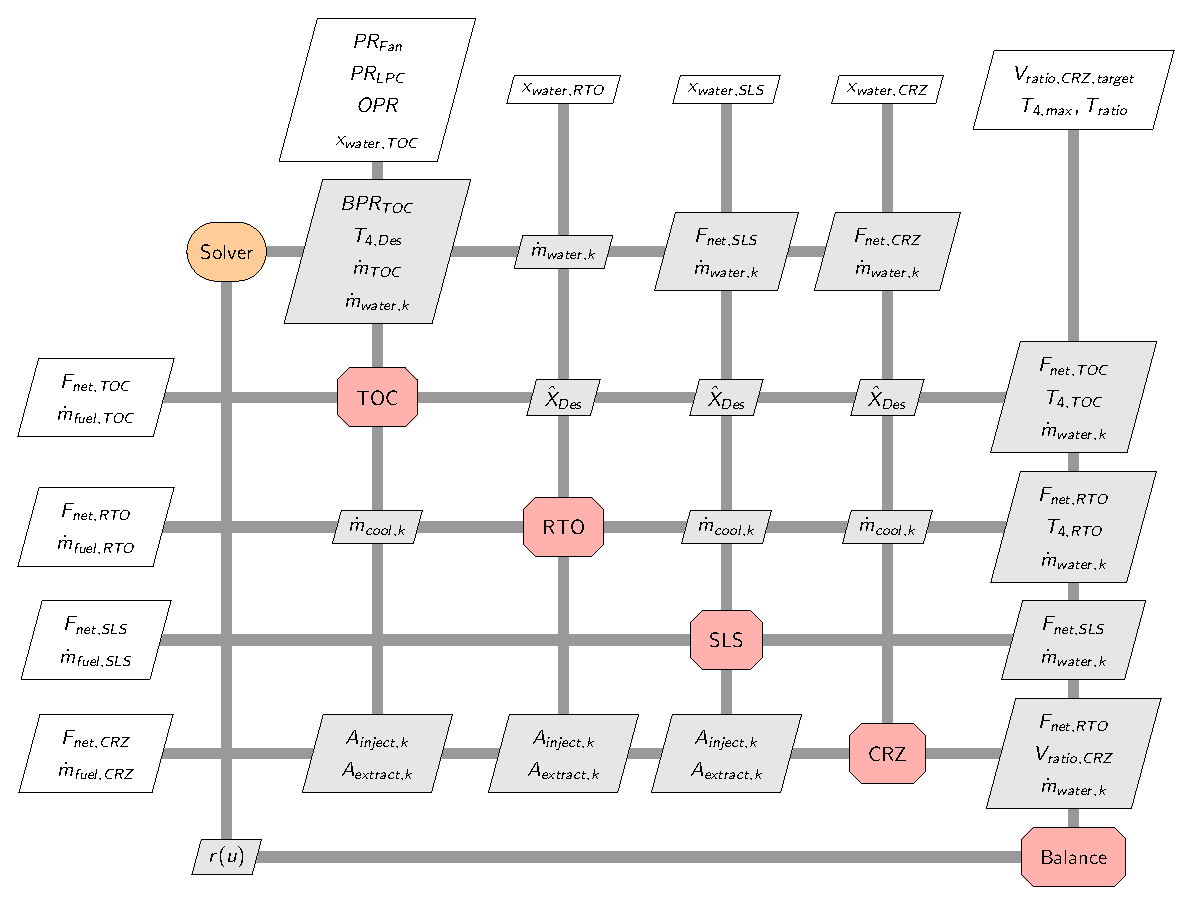
\includegraphics[width=0.75\textwidth]{N3_xdsm_full.pdf}
    \caption{
        Full model N+3 XDSM diagram.
        This XDSM diagram shows the multipoint coupling between the different operation conditions and shows how the water recovery fractions are used to solve for water mass flow rates.
    }
    \label{fig:N3_xdsm_full}
\end{figure}

% Update with table from Andrew
\begin{table}[hbt!]
    \centering
    \caption{
        N+3 engine model parameters.
        Atmospheric parameters specify the flight conditions and humidity of the atmosphere and Lower Heating Values are given for each fuel to compute TSEC.}
    \begin{tabular}{c c c c}
        \hline
        Parameter              & Value   & Units          & Comments                                        \\
        \hline
        $h_{\rm{TOC}}$         & 0.00017 & -              & humidity ratio at TOC \cite{Kalnay1996}         \\
        $h_{\rm{CRZ}}$         & 0.00017 & -              & humidity ratio at CRZ \cite{Kalnay1996}         \\
        $h_{\rm{RTO}}$         & 0.009   & -              & humidity ratio at RTO \cite{Kalnay1996}         \\
        $h_{\rm{SLS}}$         & 0.009   & -              & humidity ratio at SLS \cite{Kalnay1996}         \\
        $\rm{LHV}_{\rm{JetA}}$ & 18564.0 & \unit{BTU/lbm} & Lower heating value of Jet-A \cite{Lawicki2002} \\
        $\rm{LHV}_{\rm{H2}}$   & 51591.0 & \unit{BTU/lbm} & Lower heating value of H2 \cite{toolbox2003}    \\
        \hline
    \end{tabular}
    \label{engine_params}
\end{table}

\section{Optimization Problem}
\label{sec:optprob}

\subsection{Problem Statment}
% Briefly discuss the optimization problem
We will perform gradient-based design optimization of the engine model with the multipoint architecture that considers each of the flight conditions experienced by commercial aircraft.
% We will perform a parameter sweep of the limiting constraint to understand the impact of different emissions and performance requirements on the design space.
The objective is to minimize the TSEC since that is our performance metric for comparing the two types of fuels.
However, since we are constraining net thrust at each operating condition this optimization problem becomes ill-posed.
Therefore, we will minimize fuel flow rate, $W_{fuel}$ at the cruise condition subject to net thrust and engine diameter constraints since this will accomplish the same goal with a better posed problem.
An XDSM diagram of the optimization problem with the multipoint formulation is shown in Figure \ref{fig:N3_xdsm_opt}.

\begin{figure}[!hbt]
    \centering
    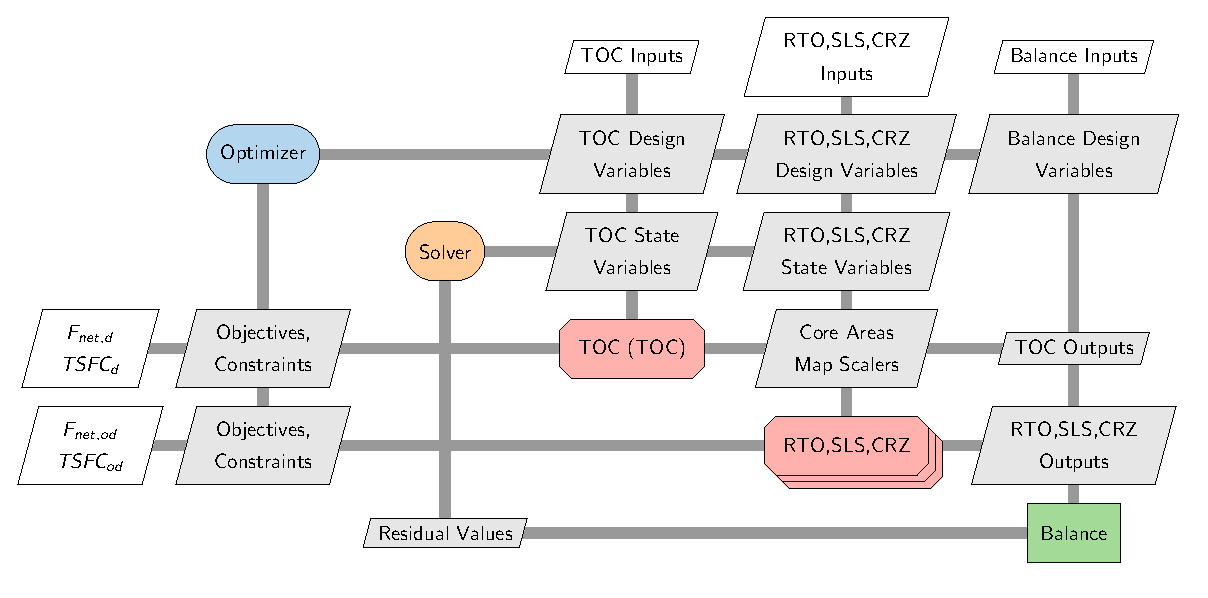
\includegraphics[width=0.75\textwidth]{N3_xdsm_opt.pdf}
    \caption{
        XDSM diagram of the multipoint optimization problem with constraints.
        The XDSM diagram shows the variables and outputs within the optimization model and how each of these values is connected to the optimizer and design points.}
    \label{fig:N3_xdsm_opt}
\end{figure}

This optimization problem was run for both Jet-A and H2 fuels using the parameters given in Table \ref{engine_params}.
The optimization problem objective function, design variables, and constraints are shown in Table \ref{tab:opt_problem} below.

% [ ] TODO: AL - PA, Define the T4 ratio with an equation and reference the equation in the table
% [ ] TODO: AL-PA, I thought we were only doing recovery fractions at CRZ??
\begin{table}[hbt!]
    \centering
    \caption{
        Multipoint optimization problem definition.
        The 4 design variables are the water recovery fractions of the core exhaust stream at each operation condition.
        The objective function is the thrust specific energy consumption at the cruise condition with a net thrust constraint at the design point, TOC.
    }
    \small
    \renewcommand{\arraystretch}{1.2}
    \begin{tabular}{r l l l l}
        \toprule
                        & Variable/Function              & Description                                 & Units            & Quantity \\
        \hline
        minimize        & $ \dot{m}_{\rm{fuel,CRZ}} $    & Fuel flow rate at CRZ                       & \unit{lbm/s}     & 1        \\
                        &                                &                                             &                  &          \\
        with respect to & $X_{\rm{H2O,TOC}}$             & Water recovery fraction at TOC              & -                & 1        \\
                        & $X_{\rm{H2O,RTO}}$             & Water recovery fraction at RTO              & -                & 1        \\
                        & $X_{\rm{H2O,SLS}}$             & Water recovery fraction at SLS              & -                & 1        \\
                        & $X_{\rm{H2O,CRZ}}$             & Water recovery fraction at CRZ              & -                & 1        \\
                        & $\rm{PR}_{\rm{HPC,TOC}}$       & TOC high-pressure compressor pressure ratio & -                & 1        \\
                        & $\rm{PR}_{\rm{LPC,TOC}}$       & TOC low-pressure compressor pressure ratio  & -                & 1        \\
                        & $\rm{PR}_{\rm{fan,TOC}}$       & TOC fan pressure ratio                      & -                & 1        \\
                        & $T_{4,\rm{ratio}}$             & TOC-to-RTO temperature ratio                & -                & 1        \\
                        & $T_{4,\rm{RTO}}$               & RTO combustor temperature                   & \unit{\degree R} & 1        \\
                        & $V_{\rm{ratio,CRZ}}$           & RTO combustor temperature                   & \unit{\degree R} & 1        \\
        \cline{3-5}
                        &                                & Total                                       &                  & 10       \\
                        &                                &                                             &                  &          \\
        subject to      & $F_{\rm{net,TOC}} \geq 5800.0$ & Target net thrust at TOC                    & \unit{lbf}       & 1        \\
                        & $D_{\rm{fan}} \leq 100$        & Maximum Fan Diameter                        & \unit{inch^2}    & 1        \\
        \cline{3-5}
                        &                                & Total                                       &                  & 2        \\
        \bottomrule
    \end{tabular}
    \label{tab:opt_problem}
\end{table}

% Blurb about PyOptSparse and SNOPT
\subsection{Optimization Software}
OpenMDAO supports the use of different optimization packages including Scipy and PyOptSparse.
PyOptSparse is an object-oriented framework for formulating and solving nonlinear constrained optimization problems.
PyOptSparse was chosen as the main optimization package for this problem due to its wide range of open-source gradient-based optimizers and integration with  \cite{Wu2020a}.

SNOPT (Sparse Nonlinear OPTimizer) was the optimizer chosen for this work.
SNOPT is a state-of-the-art optimizer used to solve large-scale optimization problems (linear and nonlinear).
The software uses a sparse SQP (sequential quadratic programming) algorithm with a limited-memory quasi-Newton approximation to the Hessian of the lagrangian.
SNOPT is particularly useful for nonlinear problems whose functions and derivatives are expensive compute.
An augmented Lagrangian merit function ensures convergence from an arbitrary point.
SNOPT allows the nonlinear constraints to be violated (if necessary) and minimizes the sum of these violations.
Due to the robustness of the algorithm, SNOPT is a perfect optimizer to solve the highly complex Multipoint systek since the pyCycle engine cycle would occasionally reach a point that is non-physical and would thus cause the solver to fail.
SNOPT is able to respond to these solver failures and backtrack to a region in the design space that is physical and continue the optimization \cite{Gill2005a}.

\section{Results}
\label{sec:results}
The 4 optimizations mentioned in the optimation problem section were run and solved.
The optimality, feasibility, and merit function for each optimization is shown plotted in Figure \ref{fig:history_clvr}.

% results of parameter sweep

% Feasibility, Optimality, Merit Func (all 4 on same plot)
% NOTE: need to clean up this plot
\begin{figure}[hbt!]
    \centering
    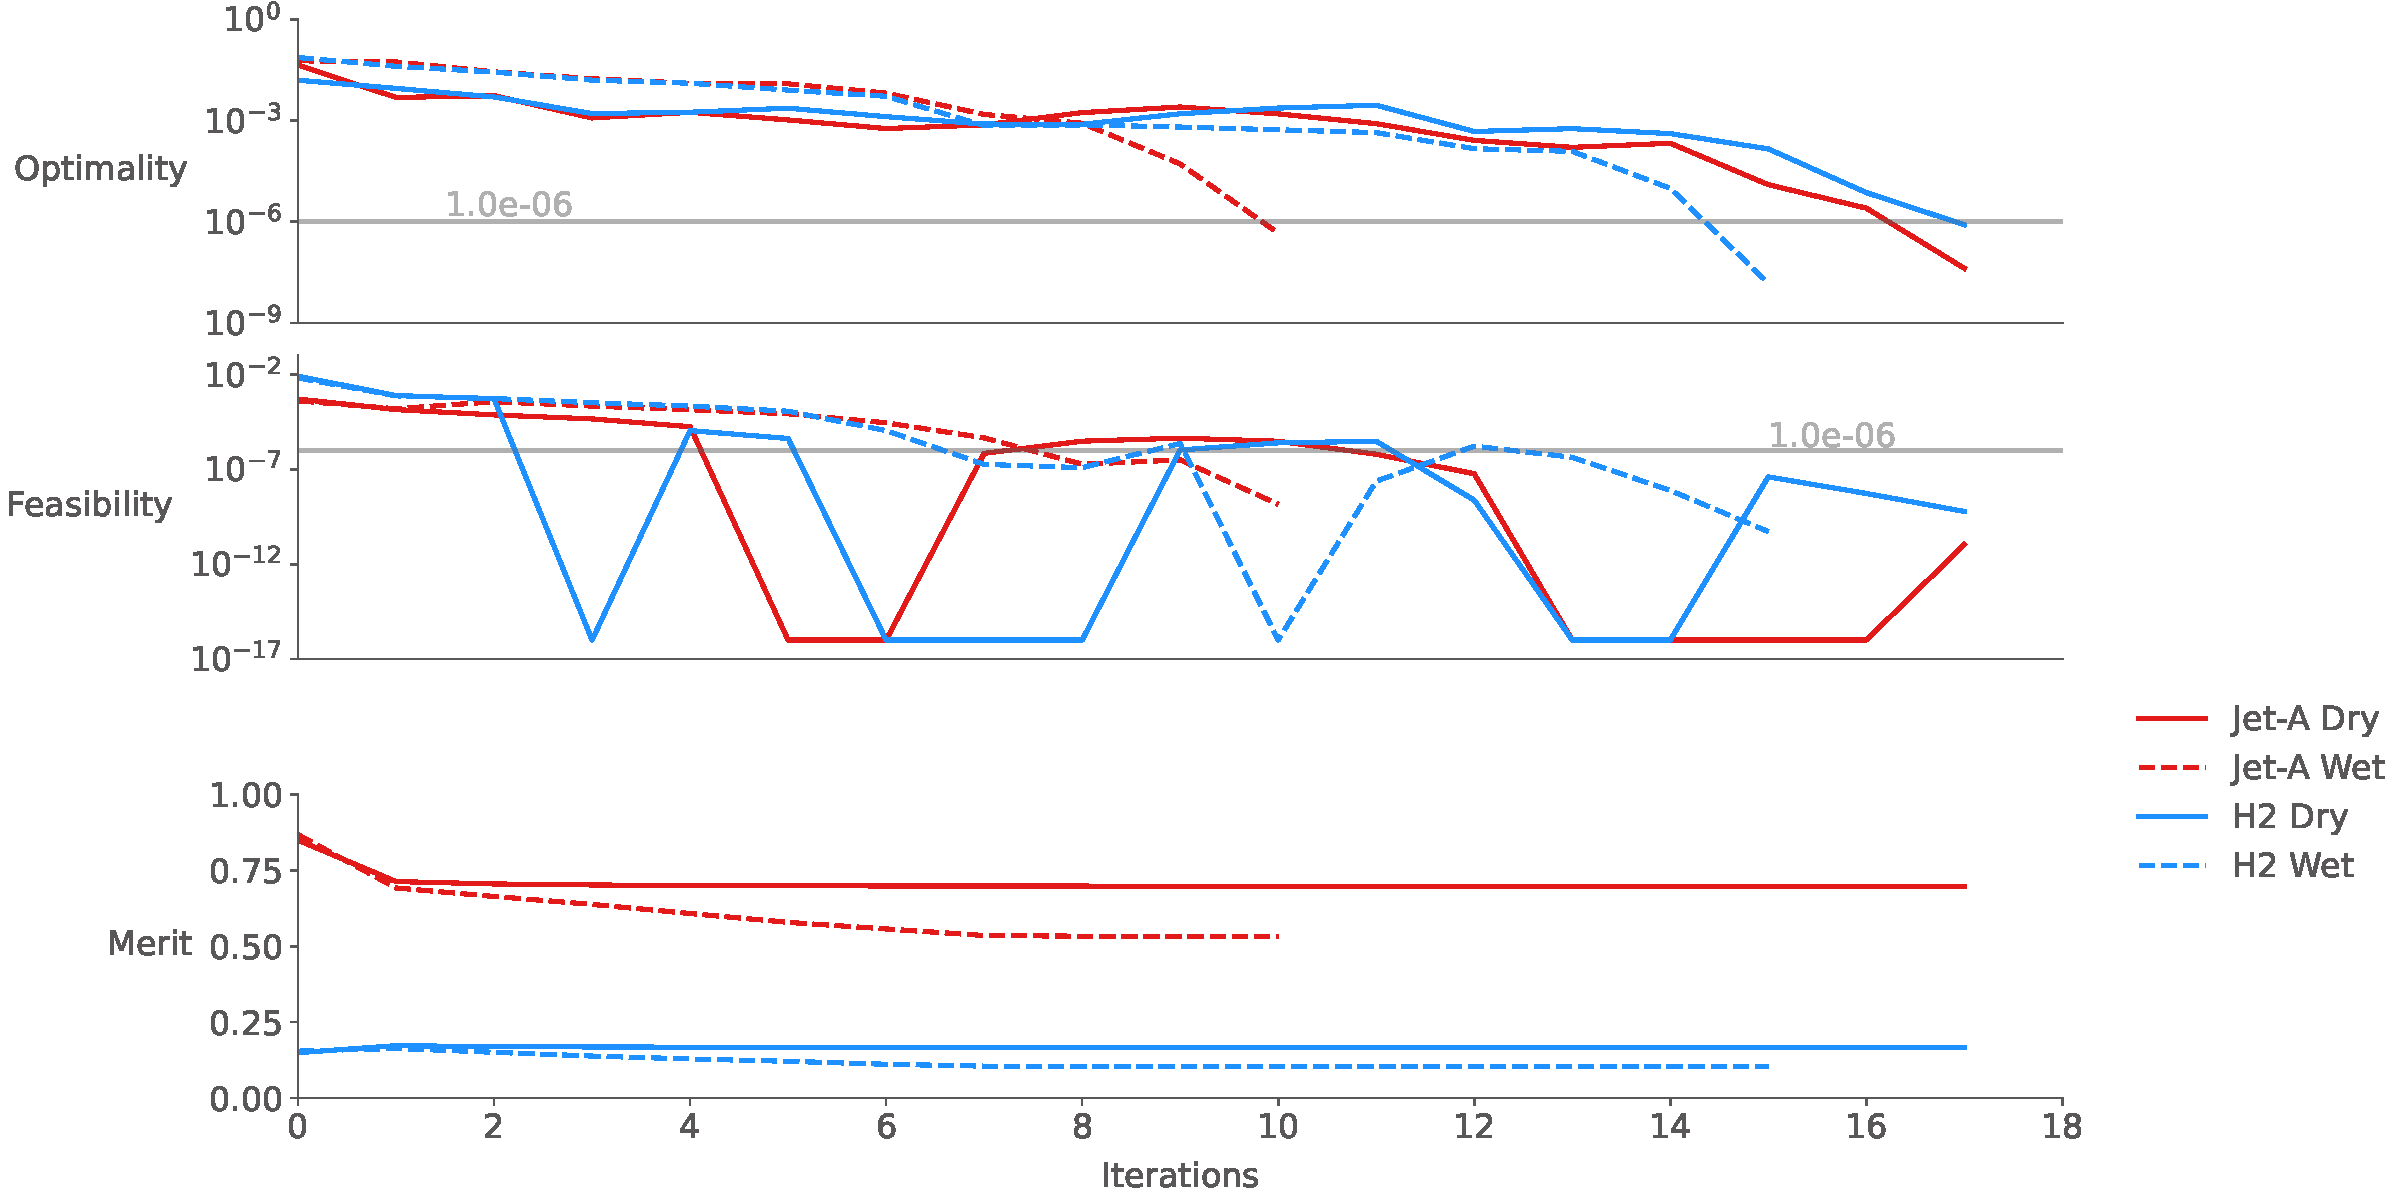
\includegraphics[width=0.8\textwidth]{opt_summary.pdf}
    \caption{The optimality, feasibility, and merit fuction for each optimization problem.
        Jet-A without water recovery is shown with the solid lines, the Jet-A with water recovery is shown with dashed lines, hydrogen without water recovery is shown with dash-dot lines, and hydrogen with water recovery is shown with dotted lines.}
    \label{fig:history_clvr}
\end{figure}

From this plot we can visually check that each optimization achieved optimality and feasibility, and that the merit function reached a steady-state value.

% DV and Constraints over each iteration

% Results of optimization problems
The optimization problems with both types of fuel but no water recovery ran smoothly and finished with 0/1 SNOPT exit codes meaning that the optimization finished successfully and met the optimiality conditions.
The resulting values of the optimization problem for Jet-A and hydrogen without water recovery are shown in Tables \ref{tab:res_thermo_opt_JetA} and \ref{tab:res_thermo_opt_H2}, respectively.
Similarly, the resulting values of the optimization problem for Jet-A and hydrogen with water recovery are shown in Tables \ref{tab:res_full_opt_JetA} and \ref{tab:res_full_opt_H2}, respectively.

% NOTE: PA - PA/AL replace this with a parallel axis plot?
% [ ] TODO: AL-PA, Yeah let's do the parallel axis plot for the basic thermodynamic parameters
% AL-PA, We can make another plot for the water fractions and the dpQp study.
\begin{table}[hbt!]
    \centering
    \caption{Optimization results of the N+3 engine with no water recovery using Jet-A as the fuel.
    }
    \small
    \renewcommand{\arraystretch}{1.2}
    \begin{tabular}{r l l l l l}
                    & Variable/Function     & Value    & Lower  & Upper & Units           \\
        \toprule
        objective   & $W_{fuel,CRZ}$        & 0.6394   & -      & -     & $\frac{lbm}{s}$ \\
        \hline
        variables   & $PR_{fan,TOC}$        & 1.285    & 1.2    & 1.4   & -               \\
                    & $PR_{LPC,TOC}$        & 4.000    & 2.5    & 4.0   & -               \\
                    & $PR_{OPR,TOC}$        & 59.495   & 40.0   & 70.0  & -               \\
                    & $T_{4,TOC}/T_{4,RTO}$ & 0.913    & 0.8    & 0.95  & -               \\
                    & $T_{4,RTO}$           & 3220.570 & -      & -     & $^\circ$R       \\
                    & $V_{ratio,CRZ}$       & 1.35     & 1.35   & 1.45  &                 \\
        \hline
        constraints & $F_{net,TOC}$         & 5800.0   & 5800.0 & -     & lbf             \\
                    & $D_{Fan}$             & 100.0    & 100    & -     & $in^2$          \\
        \bottomrule
    \end{tabular}
    \label{tab:res_thermo_opt_JetA}
\end{table}

\begin{table}[hbt!]
    \centering
    \caption{Optimization results of the N+3 engine with no water recovery using hydrogen as the fuel.
    }
    \small
    \renewcommand{\arraystretch}{1.2}
    \begin{tabular}{r l l l l l}
                    & Variable/Function     & Value   & Lower  & Upper & Units           \\
        \toprule
        objective   & $W_{fuel,CRZ}$        & 0.2331  & -      & -     & $\frac{lbm}{s}$ \\
        \hline
        variables   & $PR_{fan,TOC}$        & 1.288   & 1.2    & 1.4   & -               \\
                    & $PR_{LPC,TOC}$        & 4.000   & 2.5    & 4.0   & -               \\
                    & $PR_{OPR,TOC}$        & 59.153  & 40.0   & 70.0  & -               \\
                    & $T_{4,TOC}/T_{4,RTO}$ & 0.918   & 0.8    & 0.95  & -               \\
                    & $T_{4,RTO}$           & 3204.07 & -      & -     & $^\circ$R       \\
                    & $V_{ratio,CRZ}$       & 1.35    & 1.35   & 1.45  &                 \\
        \hline
        constraints & $F_{net,TOC}$         & 5800.0  & 5800.0 & -     & lbf             \\
                    & $D_{Fan}$             & 100.0   & 100    & -     & $in^2$          \\
        \bottomrule
    \end{tabular}
    \label{tab:res_thermo_opt_H2}
\end{table}

\begin{table}[hbt!] % need to run for T4 = 3220.570
    \centering
    \caption{Optimization results of the N+3 engine with water recovery using Jet-A as the fuel.
    }
    \small
    \renewcommand{\arraystretch}{1.2}
    \begin{tabular}{r l l l l l}
                    & Variable/Function     & Value  & Lower  & Upper & Units           \\
        \toprule
        objective   & $W_{fuel,CRZ}$        & 0.6037 & -      & -     & $\frac{lbm}{s}$ \\
        \hline
        variables   & $x_{H2O,TOC}$         & 0.115  & 0.0    & -     & -               \\
                    & $x_{H2O,RTO}$         & 0.0    & 0.0    & -     & -               \\
                    & $x_{H2O,SLS}$         & 0.0    & 0.0    & -     & -               \\
                    & $x_{H2O,CRZ}$         & 0.3    & 0.0    & 0.3   & -               \\
                    & $PR_{fan,TOC}$        & 1.291  & 1.2    & 1.4   & -               \\
                    & $PR_{LPC,TOC}$        & 4.0    & 2.5    & 4.0   & -               \\
                    & $PR_{OPR,TOC}$        & 54.218 & 40.0   & 70.0  & -               \\
                    & $T_{4,TOC}/T_{4,RTO}$ & 0.923  & 0.8    & 0.95  & -               \\
                    & $T_{4,RTO}$           & 3400.0 & -      & -     & $^\circ$R       \\
                    & $V_{ratio,CRZ}$       & 1.35   & 1.35   & 1.45  &                 \\
        \hline
        constraints & $F_{net,TOC}$         & 5800.0 & 5800.0 & -     & lbf             \\
                    & $D_{Fan}$             & 100.0  & 100    & -     & $in^2$          \\
        \bottomrule
    \end{tabular}
    \label{tab:res_full_opt_JetA}
\end{table}

\begin{table}[hbt!]
    \centering
    \caption{Optimization results of the N+3 engine with water recovery using hydrogen as the fuel.
    }
    \small
    \renewcommand{\arraystretch}{1.2}
    \begin{tabular}{r l l l l l}
                    & Variable/Function     & Value   & Lower  & Upper & Units           \\
        \toprule
        objective   & $W_{fuel,CRZ}$        & -       & -      & -     & $\frac{lbm}{s}$ \\
        \hline
        variables   & $x_{H2O,TOC}$         & 0.066   & 0.0    & -     & -               \\
                    & $x_{H2O,RTO}$         & 0.0     & 0.0    & -     & -               \\
                    & $x_{H2O,SLS}$         & 0.0     & 0.0    & -     & -               \\
                    & $x_{H2O,CRZ}$         & 0.17    & 0.0    & 0.17  & -               \\
                    & $PR_{fan,TOC}$        & 1.291   & 1.2    & 1.4   & -               \\
                    & $PR_{LPC,TOC}$        & 4.0     & 2.5    & 4.0   & -               \\
                    & $PR_{OPR,TOC}$        & 55.132  & 40.0   & 70.0  & -               \\
                    & $T_{4,TOC}/T_{4,RTO}$ & 0.927   & 0.8    & 0.95  & -               \\
                    & $T_{4,RTO}$           & 3204.07 & -      & -     & $^\circ$R       \\
                    & $V_{ratio,CRZ}$       & 1.35    & 1.35   & 1.45  &                 \\
        \hline
        constraints & $F_{net,TOC}$         & 5800.0  & 5800.0 & -     & lbf             \\
                    & $D_{Fan}$             & 100.0   & 100    & -     & $in^2$          \\
        \bottomrule
    \end{tabular}
    \label{tab:res_full_opt_H2}
\end{table}

\begin{figure}[hbt!]
    \centering
    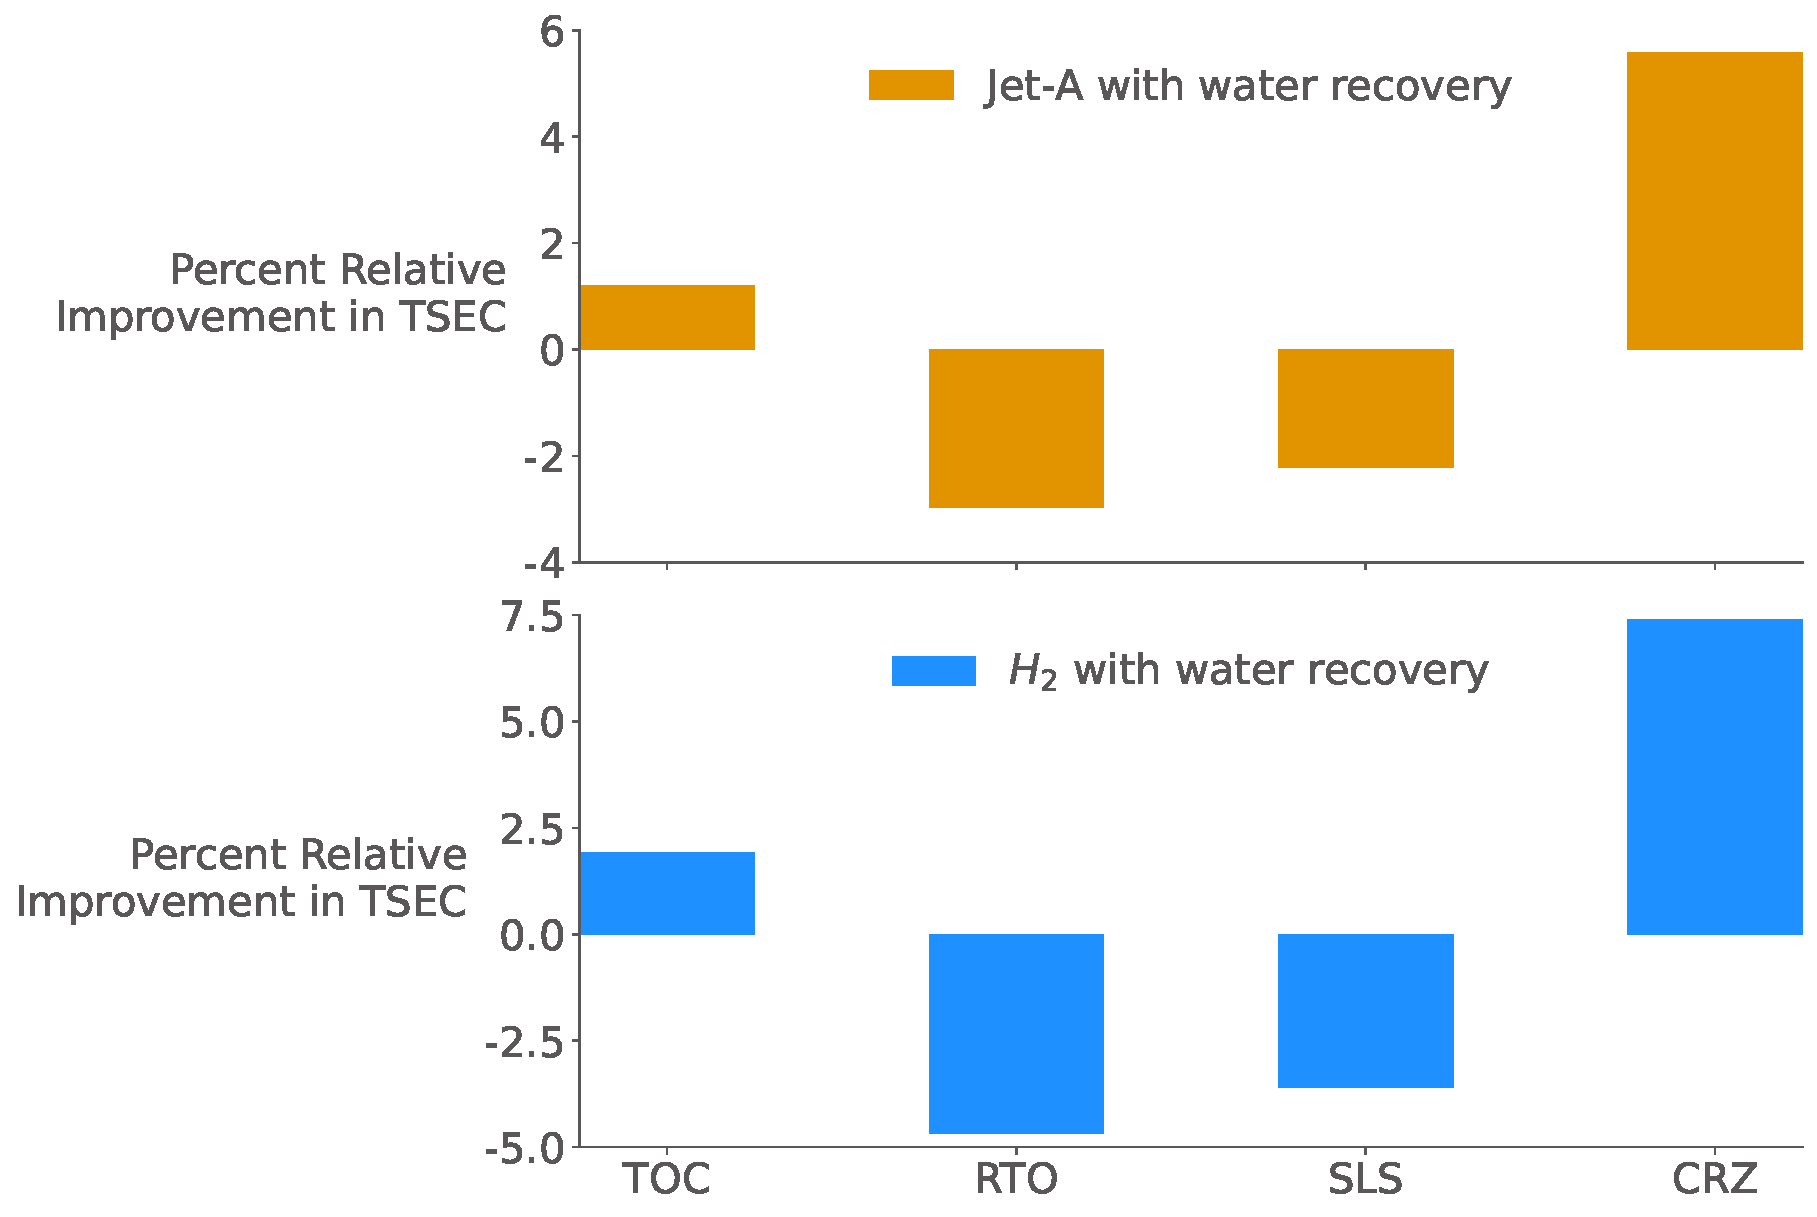
\includegraphics[width=0.8\textwidth]{JetA-H2_TSEC_diff.pdf}
    \caption{Percent relative improvement in thrust specific energy consumption (TSEC) of the N+3 engine with water recovery.
        This plot compares the relative improvement of the two optimziation problems with water recovery compared to the optimzation problems without water recovery.}
    \label{fig:barchart}
\end{figure}

% Thrust splits
% TODO PA - PA: Add thrust splits for each opt

% TSEC as a function of dPqP
% NOTE: need to clean up this plot
\begin{figure}[hbt!]
    \centering
    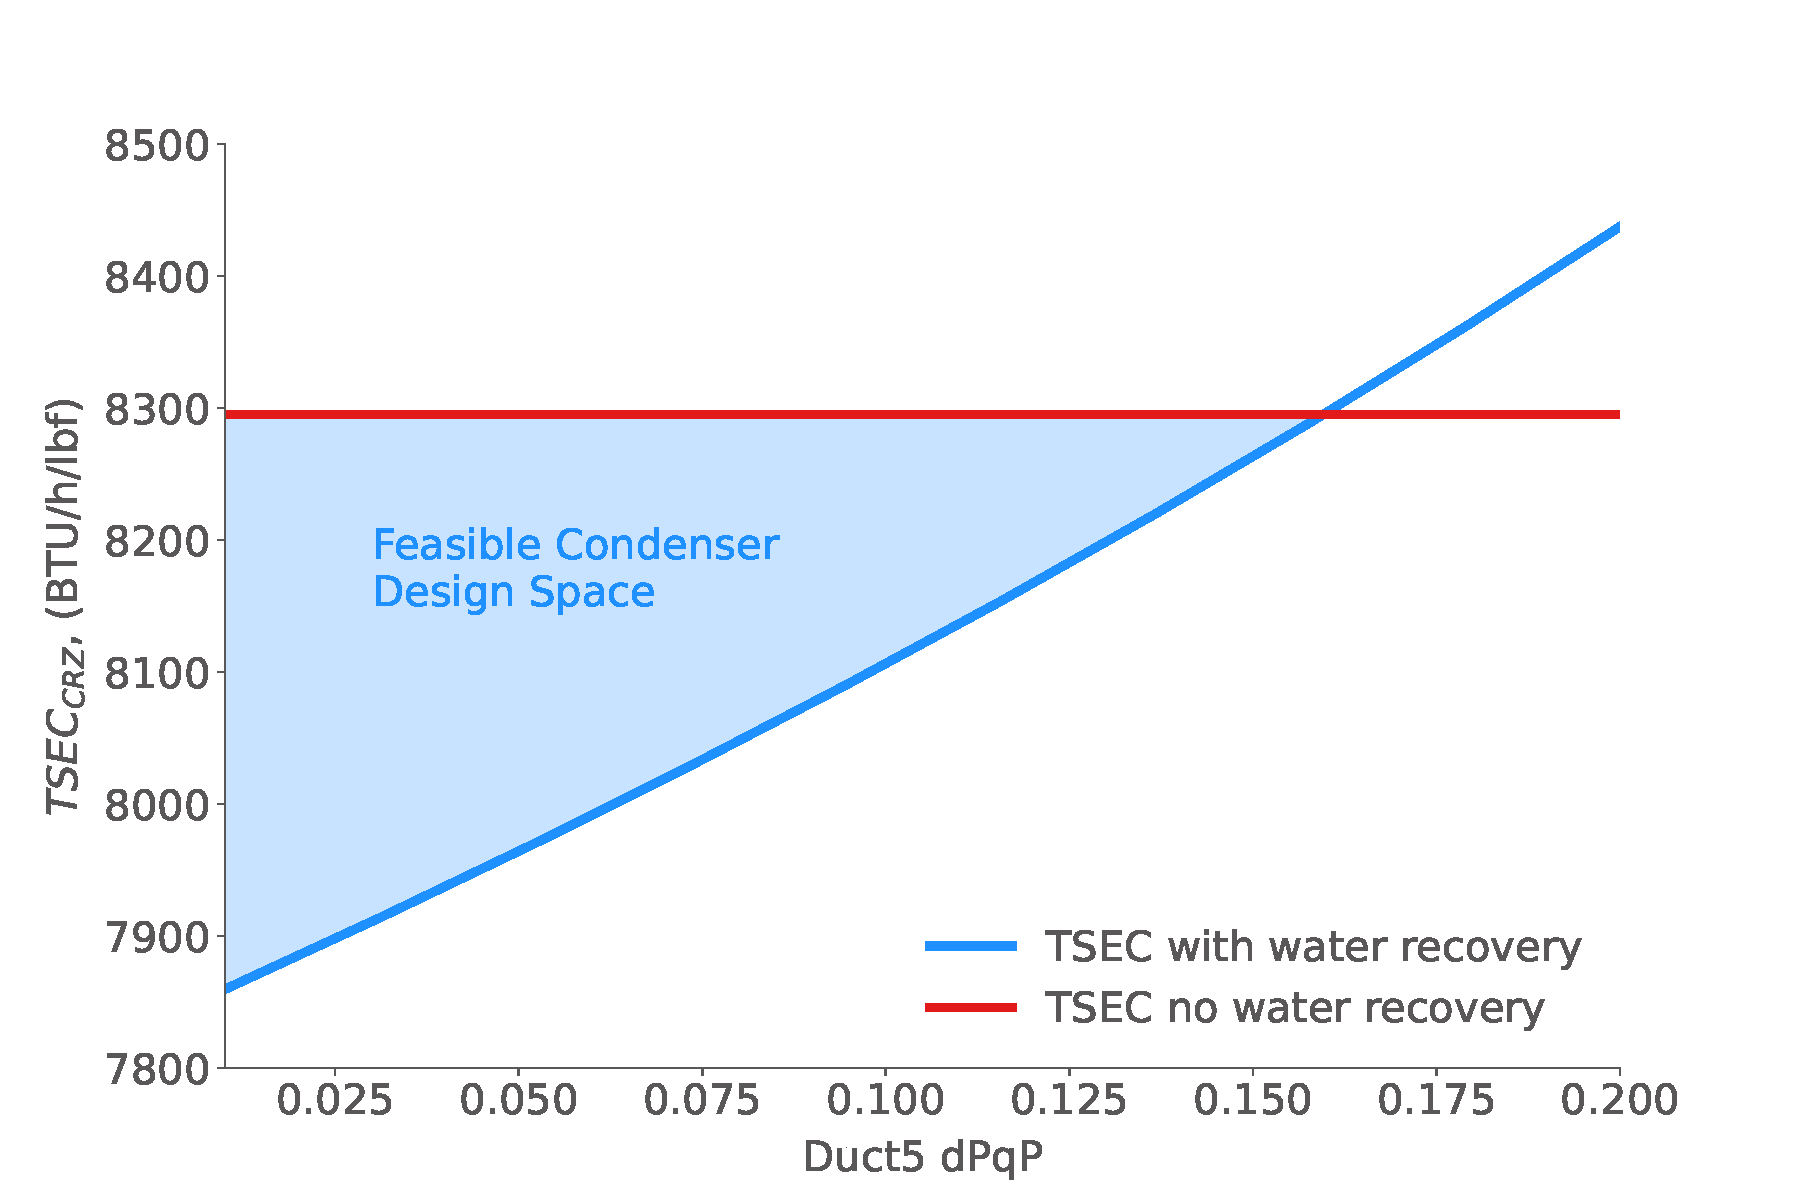
\includegraphics[width=0.8\textwidth]{N3_dpqp.pdf}
    \caption{Pressure loss sweep of Duct5 which is just upstream of the water vapor extractor component.
        The figure shows the optimized TSEC values for varying levels of pressure loss due to the condensation of water compared to the optimzation problem without water recovery.
        This shows the working space available for designing a water condensor while still gaining the benefits of water recovery.}
    \label{fig:dpqp_sweep}
\end{figure}

% Motivation: space to work with hydrogen, benefits of water injection, benefits of H2

\section{Conclusion}
\label{sec:conc}
% Message 1: Re-state the problem
% Message 2: Summarize the HBTF model
% Message 3: Expected results

\section{Acknowledgements}

\bibliography{mdolab,references}

\end{document}